% SIAM Article Template
\documentclass[review,onefignum,onetabnum]{siamart190516}

% Information that is shared between the article and the supplement
% (title and author information, macros, packages, etc.) goes into
% ex_shared.tex. If there is no supplement, this file can be included
% directly.

% SIAM Shared Information Template
% This is information that is shared between the main document and any
% supplement. If no supplement is required, then this information can
% be included directly in the main document.


% Packages and macros go here
\usepackage{lipsum}
\usepackage{amsfonts}
\usepackage{graphicx}
\usepackage{epstopdf}
\usepackage{algorithmic}
\usepackage{bookmark}
\ifpdf
  \DeclareGraphicsExtensions{.eps,.pdf,.png,.jpg}
\else
  \DeclareGraphicsExtensions{.eps}
\fi

% Add a serial/Oxford comma by default.
\newcommand{\creflastconjunction}{, and~}

% Used for creating new theorem and remark environments
\newsiamremark{remark}{Remark}
\newsiamremark{hypothesis}{Hypothesis}
\crefname{hypothesis}{Hypothesis}{Hypotheses}
\newsiamthm{claim}{Claim}


% Title. If the supplement option is on, then "Supplementary Material"
% is automatically inserted before the title.
\title{18.335 Final Project Report}
\author{Juan M Ortiz}


\usepackage{amsopn}
\DeclareMathOperator{\diag}{diag}

% Packages
\usepackage{enumitem}

% Optional PDF information
\ifpdf
\hypersetup{
  pdftitle={18.335 Final Project Report},
  pdfauthor={Juan M Ortiz}
}
\fi

\begin{document}
\maketitle

% REQUIRED
\begin{abstract}
  \lipsum[1]
\end{abstract}

\section{Introduction}
Along with the numerous benefits that we have come to enjoy in our transition to the Digital Age
have come a plethora of technical challenges. In particular, the rise in the prominence
of the role that data plays in our services has forced us to invent efficient solutions 
to challenges related to storing, retrieving, processing, and transmitting various types of 
data. One of the most common types of data that we utilize in both computer and mobile environments
is that of images. As such, there has been a lot of research in the field of image compression.
Although the problem of compressing images falls within the general problem of compressing arbitrary
raw binary data, we can greatly improve our performance by designing encoders that take 
advantage of the statistical properties that images posses. Through the use of our domain-specific
knowledge about how images are composed as well as how we perceive images, 
modern compression algorithms are able to remove a great deal of redundancies
so as to create much smaller representations that are able to be decoded into 
good reconstructions of the originals in accordance to human visual perception.

\subsection{Compression Principles}

Today, the majority of methods utilized in image compression are based on the
principles of \textbf{entropy coding} and \textbf{transform coding}. 

The first, entropy coding, refers to a type of lossless compression scheme which is not
dependent on the medium to which it is applied. Entropy coding aims to reduce
the size of data processed by defining a mapping between the original symbols/patterns of 
the data to one in which frequently occurring symbols/patterns are represented 
using few bits and those that occur rarely are represented with more bits.
The two most common algorithms used for entropy coding are Huffman coding and
Arithmetic coding. A more detail overview of Huffman coding will be given in \textbf{Section 2}. On the other hand, transform coding refers to a technique utilized when dealing
with natural data sources such as images and audio. The main idea behind transform
coding is to utilize a linear process to convert the original representation of
the data to one in which the most relevant information is contained within
a few coefficients. On its own, a naive transform coding approach is lossless and 
does not significantly reduce the information needed to encode the original data. However,
the new representation along with domain knowledge about the data being encoded 
enables us to keep only the most relevant information to recreate something that is mostly
faithful with the original but is much smaller. The most widely used transform coding algorithm when
dealing with image compression is that of the discrete cosine transform (DCT) which
will be further described in \textbf{Section 2}. Additionally, we will describe
a method based on the singular value decomposition (SVD) and compare it against
the commonly used DCT.

\subsection{Modules of Image Coder}
The typical configuration of an image encoder system is composed of the following 
modules: source encoder, quantizer, and entropy coder \cite{raid2014jpeg}. A brief
description of each of these modules is provided below:

\begin{enumerate}[label=\textbf{(\alph*)}]
  \item \textbf{Source Encoder.} 
  The purpose of this module in the encoder system is to decorrelate the original
  input and transform it into a set of sparse data values through the use of a 
  transform coding method. In doing so, the new data representation compacts the
  information of the original data into a small number of coefficients.

  \item \textbf{Quantizer.}
  The goal of the quantizer module is to reduce the amount of information needed
  to store the representation created by the source encoder through decreasing 
  the precision of the coefficients of the representation. During this step,
  we can take advantage of domain-knowledge to discard information that will not
  significantly affect the reconstruction of the input data.

  \item \textbf{Entropy Coder.}
  The last step in a typical compression system is the entropy coder module.
  This step in the compression is lossless and aims to remove redundancies in the
  bit-patterns produced by the quantized output of the quantizer module.
\end{enumerate}

\begin{figure}[tbhp]
  \centering
  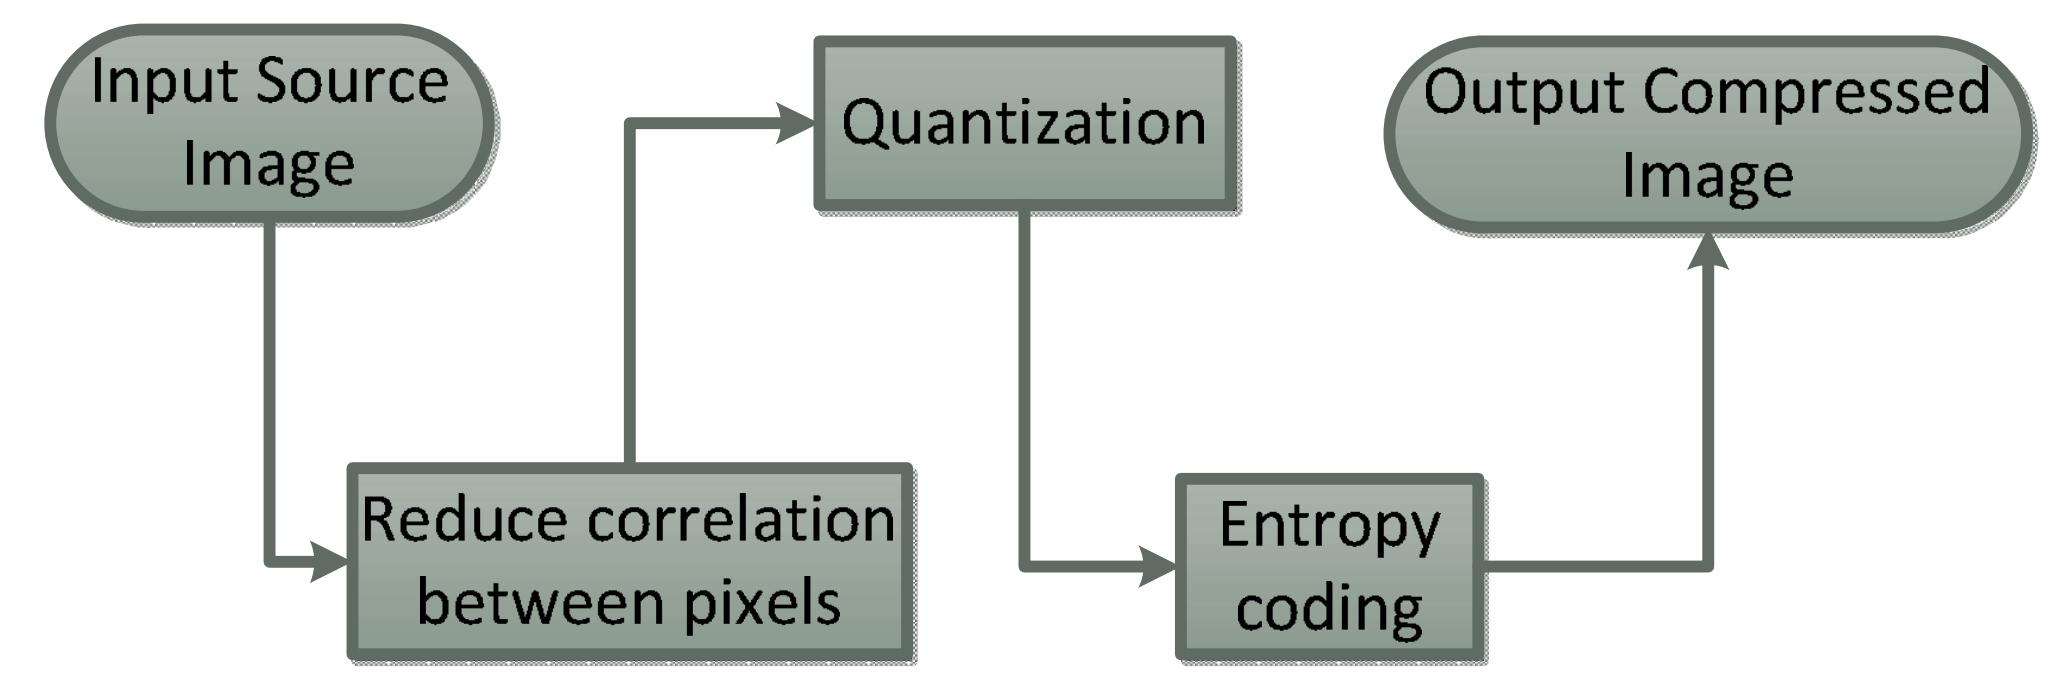
\includegraphics[width=0.9\textwidth]{compression system.png}
  \caption{Typical Compression System Architecture from \cite{raid2014jpeg}}
  \label{fig:compression-arch}
\end{figure}

\subsection{Evaluation Metrics}
\lipsum[10-11]

\section{Background}
\subsection{Explanation}
\lipsum[12]

\subsection{Color Specification}
\lipsum[13-14]

\subsection{Discrete Cosine Transform}
\cite{ahmed1974discrete}
\lipsum[15-18]

\subsection{Singular Value Decomposition | Low Rank Approximation}
\lipsum[10-20]

\subsection{Block Algorithms}
\lipsum[21-23]

\subsection{Huffman Coding}
\lipsum[24-25]

\section{Experiments}
\subsection{Image Quality}
Need to test the ability of the algorithms to reconstruct the original image 
over different settings.

Possibly compare the reconstruction accuracy vs the compression

\lipsum[26-30]

\subsection{Performance}
Compare compression vs operations
compare quality vs operations

\lipsum[31-32]

\section{Conclusion}
Nice ass conclusion

\lipsum[33-34]

\pagebreak
\bibliographystyle{siamplain}
\bibliography{references}
\end{document}
